% INTRODUCTION

\section{Nucleon Spin: Valence and Sea Quark Polarization}
\label{sec:introduction}
The last two decades has seen remarkable progress in the knowledge 
of the polarized parton distribution functions (pPDF)
  $\Delta q_f(x)$.
The most precise and clearly interpreted data are from inclusive deep-inelastic
 lepton scattering (DIS)
experiments at CERN and SLAC. 
However, the information available from inclusive DIS process has inherent 
limitations.  As the cross 
sections are only sensitive to $e_q^2$, the quark charge square,
an inclusive experiment probes quarks and anti-quarks on an equal footing, and
 it is only possible to determine combinations of $\Delta q + \Delta \bar{q}$, 
but never the valence $\Delta q_v=\Delta q - \Delta \bar{q}$ nor the sea $\Delta \bar{q}$ separately.    
 Therefore it is not sensitive to the symmetry breaking in the sea sector. 
Through inclusive DIS measurements, only one particular flavor non-singlet can be directly 
inferred  i.e.  $\Delta q_{3}(x,Q^2)=\Delta u+\Delta \bar{u}-\Delta d-\Delta \bar{d}$. 
The additional assumption of SU(3)$_f$ flavor symmetry allows the hyperon beta decay data
to constrain the first moments of $\Delta q$.
The well-cited result of this approach is
that quark helicities seem to make a small net contribution to the nucleon spin, and the
strange sea appears to be negatively polarized.

Are sea quarks polarized ?  Do sea quarks' polarization have a flavor asymmetry similar to that of  their unpolarized part ?  
  How much do sea quarks polarization  (helicity) contribute to nucleon's 1/2-spin ? 
These question has been tantalizing us for the last  two decades.   From inclusive deep-inelastic spin asymmetry measurements, combined with hyperon decay data assuming  SU(3) symmetry, it was suggested that sea quarks' polarization are negative~\cite{Blumlein:2010rn},  contributing about $10\%$ of nucleon's spin.  
%cite smc, slac, spin crisis.
 However,  semi-inclusive DIS data from SMC~\cite{Adeva:1997qz}, HERMES ~\cite{Airapetian:2004zf}, and COMPASS~\cite{Alekseev:2010ub} experiment concluded that sea quark's polarization are consistent with zero,  as shown in Fig.~\ref{fig:pdgpolq},  and that sea quarks' polarization do not have a flavor asymmetry.
 % \cite  

The sensitivity to each individual quark flavor can also be realized
in semi-inclusive deep inelastic scattering (SIDIS)
in which one of the leading hadrons in quark fragmentation is also detected.
Since the leading hadrons from the current fragmentation 
carry information about
the struck quark's flavor, detection of the leading hadron 
effectively ``tags'' the quark flavor.
Therefore, SIDIS offers an unique opportunity 
for determining the spin, flavor, and sea structure of the nucleon \cite{Frankfurt}, 
thereby significantly enriching 
our understanding of QCD and the nucleon structure. 
High precision polarized SIDIS data on the proton and the neutron 
(in a deuteron or a $^3$He nuclei) allows
a flavor decomposition of nucleon spin structure, which could lead to
the discovery of a possible flavor-asymmetry in the polarized sea.
A decade ago, in 2004, the HERMES collaboration
published the results of a leading order spin flavor decomposition from polarized 
proton and deuteron data, and extracted the sea quark 
polarizations~\cite{Airapetian:2004zf}  for the first time without assuming  flavor symmetry of polarized sea. Unlike 
the predictions of several theoretical models,
HERMES data indicated that within the available statistics
$\Delta \bar{u}- \Delta \bar{d}$ is consistent
with an unbroken SU(2)$_f$ symmetry.  These results have been confirmed in 2010 by the COMPASS Collaboration~\cite{Alekseev:2010ub},   as shown in Fig.\ref{fig:polubardbar}. 
%xj.  add citation COMPASS and comments here.  

\begin{figure} [htbp]
  \centering
    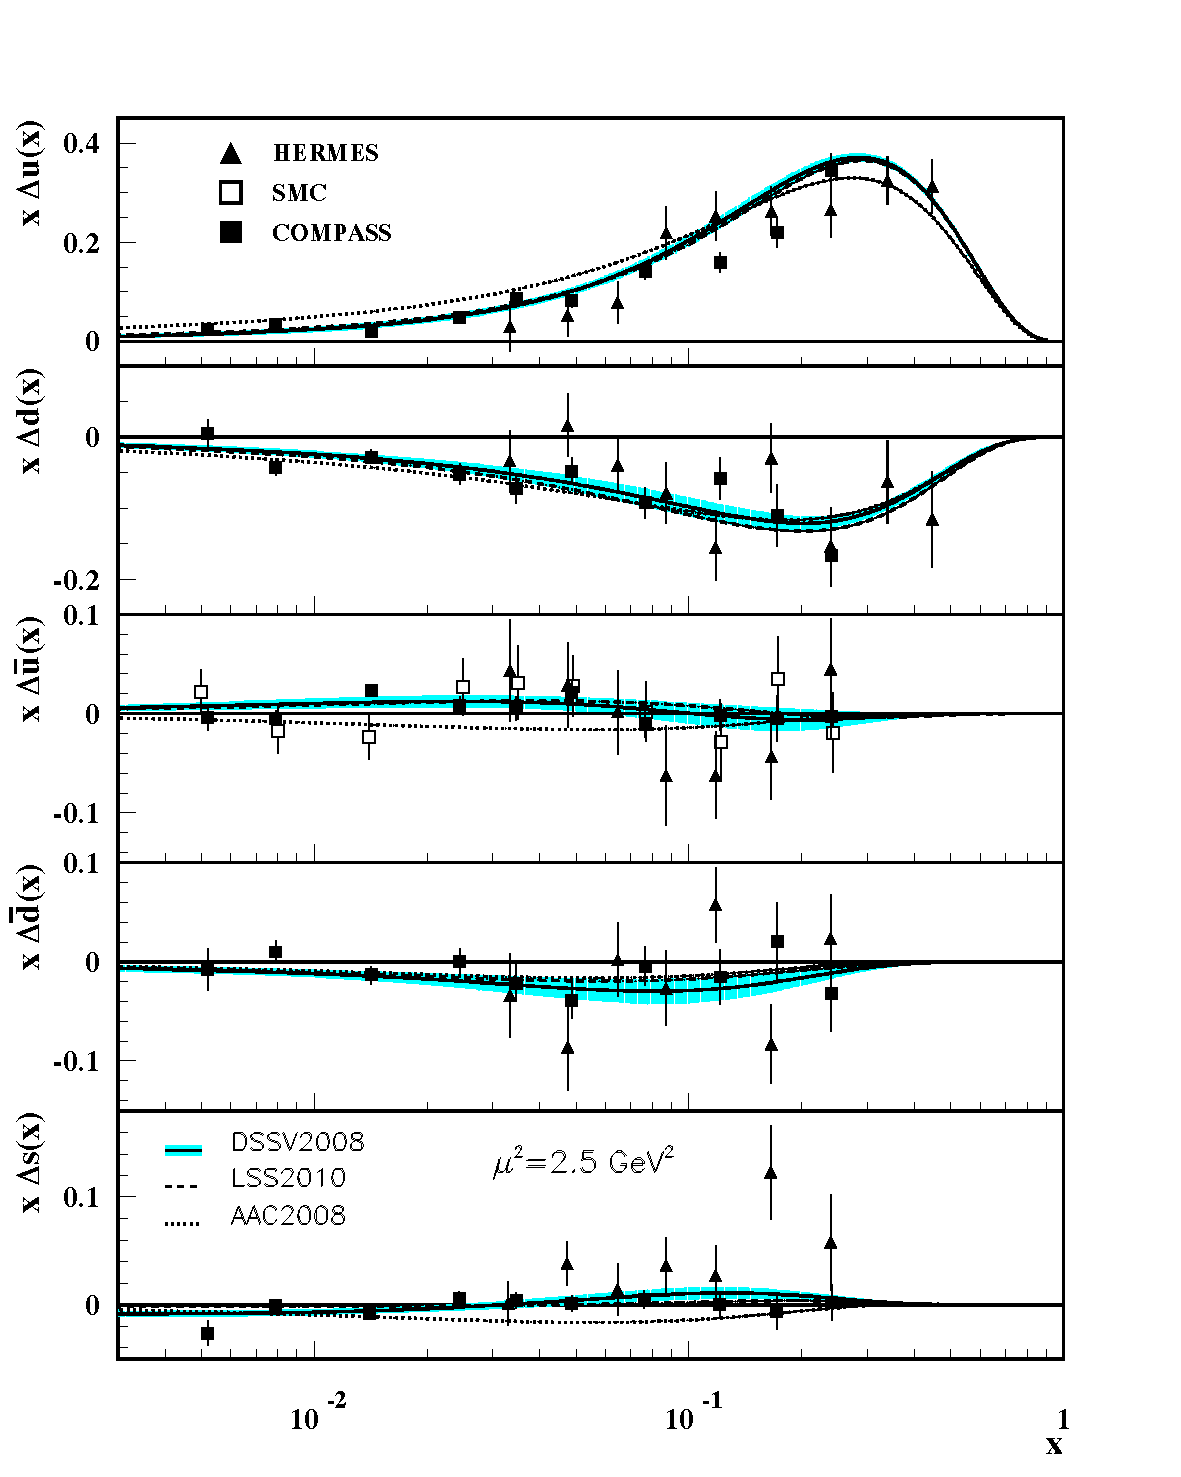
\includegraphics[width=0.80\linewidth]{figs_xj/pdg_polq2013.pdf}
  \caption{\label{fig:pdgpolq}  From Particle Data Group (2013).  As extracted from SIDIS data on proton and deuteron targets, distributions of x times the polarized parton distributions $\Delta q(x)$ (where $q = u, d, \bar{u}, \bar{d}, s$),   using the LSS2010~\cite{Leader:2010rb}, AAC2008~\cite{Hirai:2008aj}, and DSSV2008~\cite{DSSV2008}
parameterizations at a scale $\mu^2 = 2.5$ GeV$^2$, showing the error corridor of the latter set (corresponding to a one-unit increase in $\chi^2$). Points represent data from semi-inclusive positron (HERMES~\cite{Airapetian:2004zf}) and muon (SMC~\cite{Adeva:1997qz}
and COMPASS ~\cite{Alekseev:2010ub}) deep inelastic scattering given at $Q^2 = 2.5$ GeV$^2$. SMC
results are extracted under the assumption that $\Delta \bar{u}(x) = \Delta \bar{d}(x)$. }
\end{figure}

\begin{figure} [htbp]
  \centering
    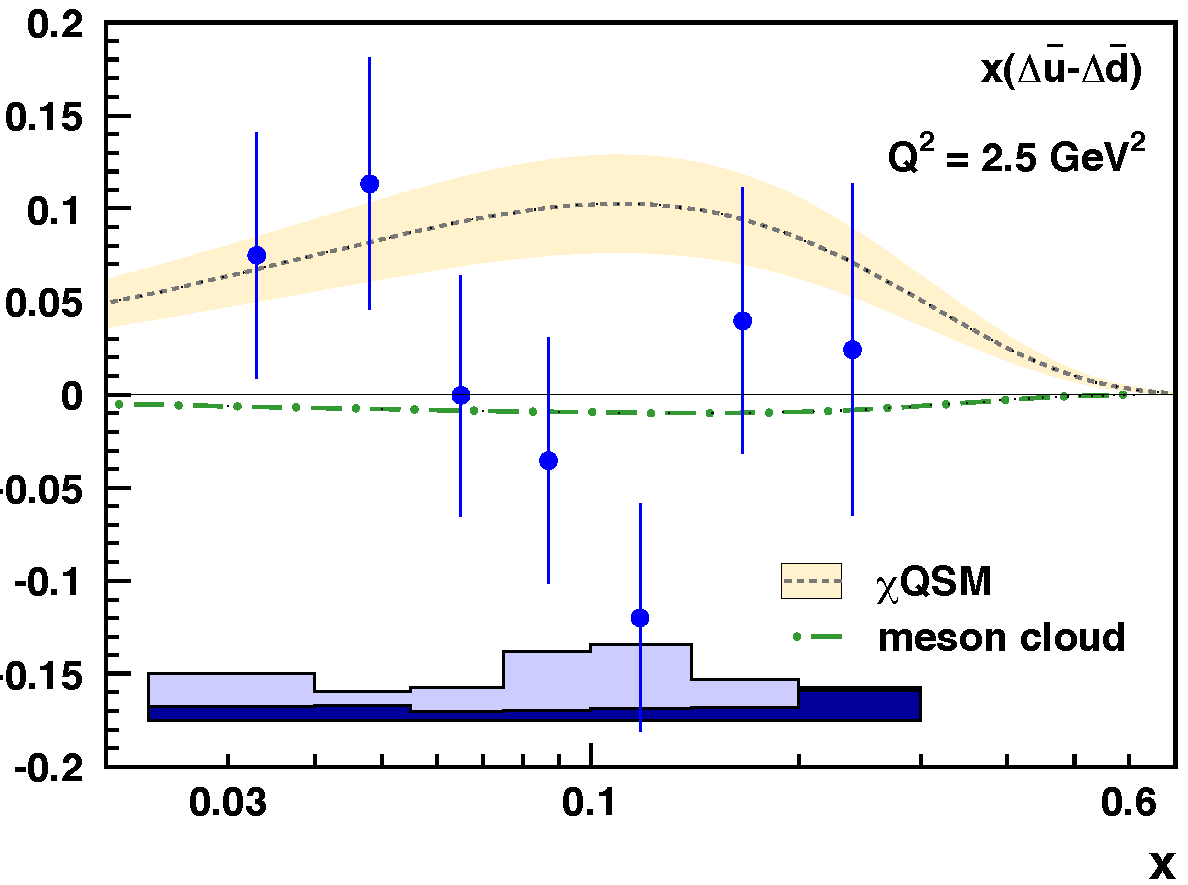
\includegraphics[width=0.41\linewidth]{figs_xj/hermes_dubar_ddbar2005.pdf}
    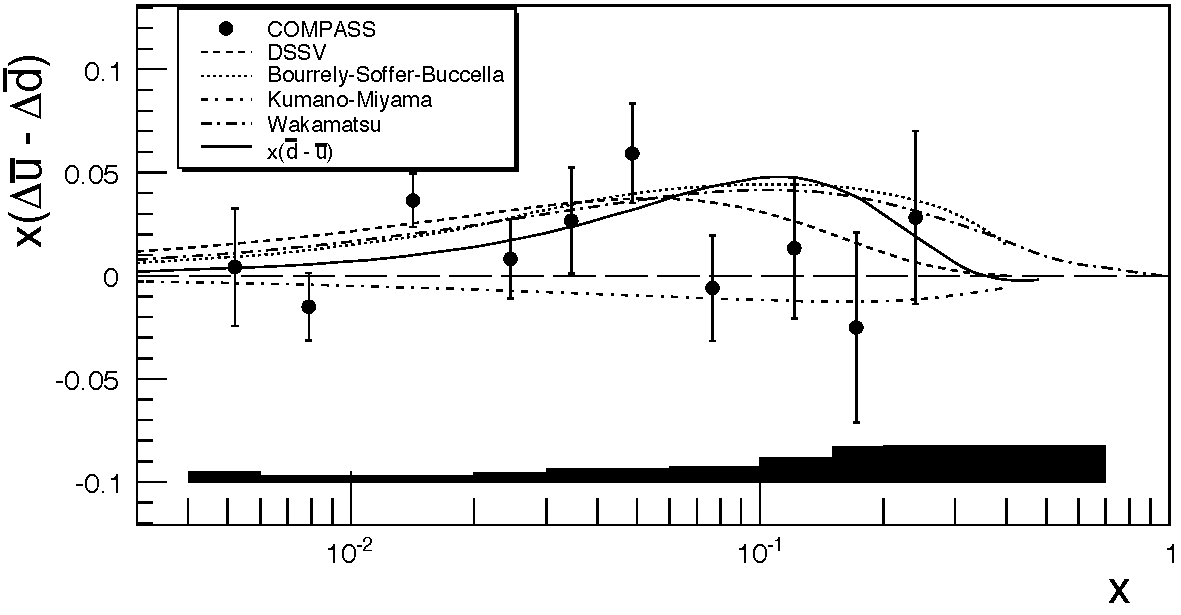
\includegraphics[width=0.58\linewidth]{figs_xj/compass_dbar_ubar2010.pdf} \\
  \caption{\label{fig:polubardbar} 
  The HERMES result~\cite{Airapetian:2004zf} of 
 polarized sea flavor asymmetry
$x(\Delta \bar{u} - \Delta \bar{d})$ is shown on the left, COMPASS result~\cite{Alekseev:2010ub} is shown on the right.
The error bars are statistical, while the shaded bands at the bottom indicate the systematic
uncertainties.}
\end{figure}

Very recently, from RHIC STAR experiment's W-boson spin asymmetry measurements~\cite{Adamczyk:2014xyw}, as shown in Fig~\ref{fig:STAR_W}, the data strongly favor a positively polarized sea up-quark.  
The STAR data agree reasonably well when compared with the Statistical Model (BBS2008) ~\cite{Bourrely200739}, in which a sea up-quark polarization as large as $~20\%$, as shown in Fig.\ref{fig:STAR_W} right-panel.
% add more comments, and a figure here.
% STAR W paper and ubar positive polarization.
%%% Fig %%%

\begin{figure} [htbp]
  \centering
    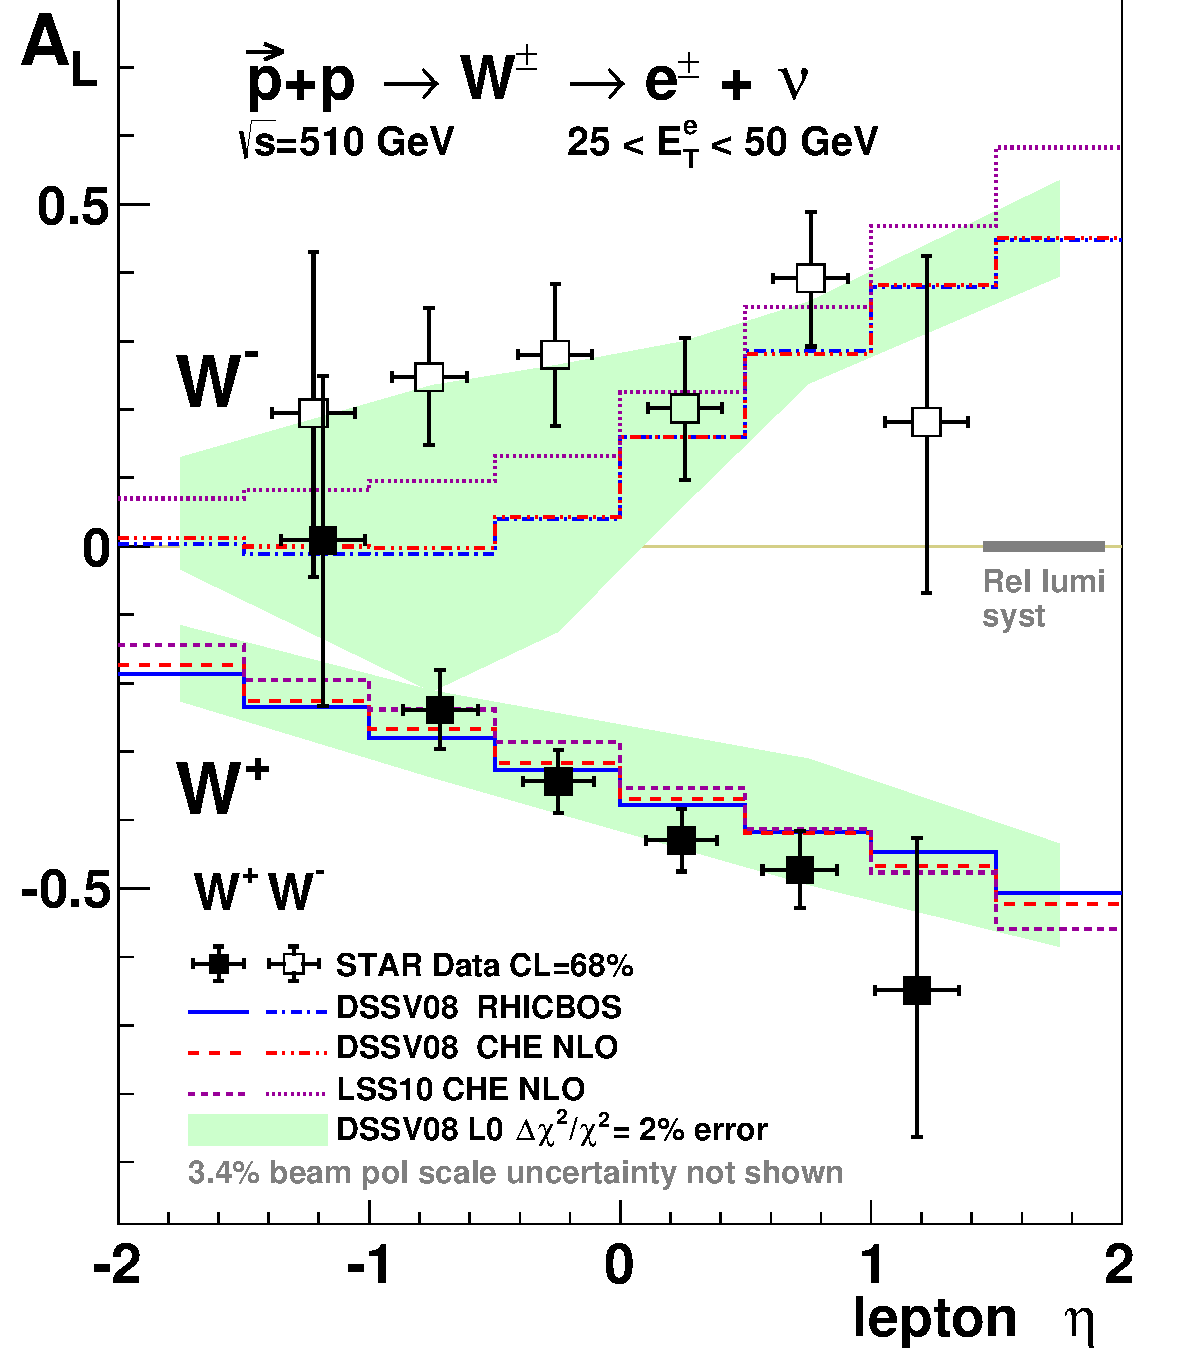
\includegraphics[width=0.60\linewidth]{figs_xj/STAR-WAL_2012.pdf}
  \caption{\label{fig:STAR_W} Recent results from STAR~\cite{Adamczyk:2014xyw},  longitudinal single-spin asymmetry, $A_L$, for $W^\pm$ production as a function of lepton pseudorapidity, $\eta_e$, in comparison with theory predictions. 
 }
\end{figure}

\begin{figure} [htbp]
  \centering
    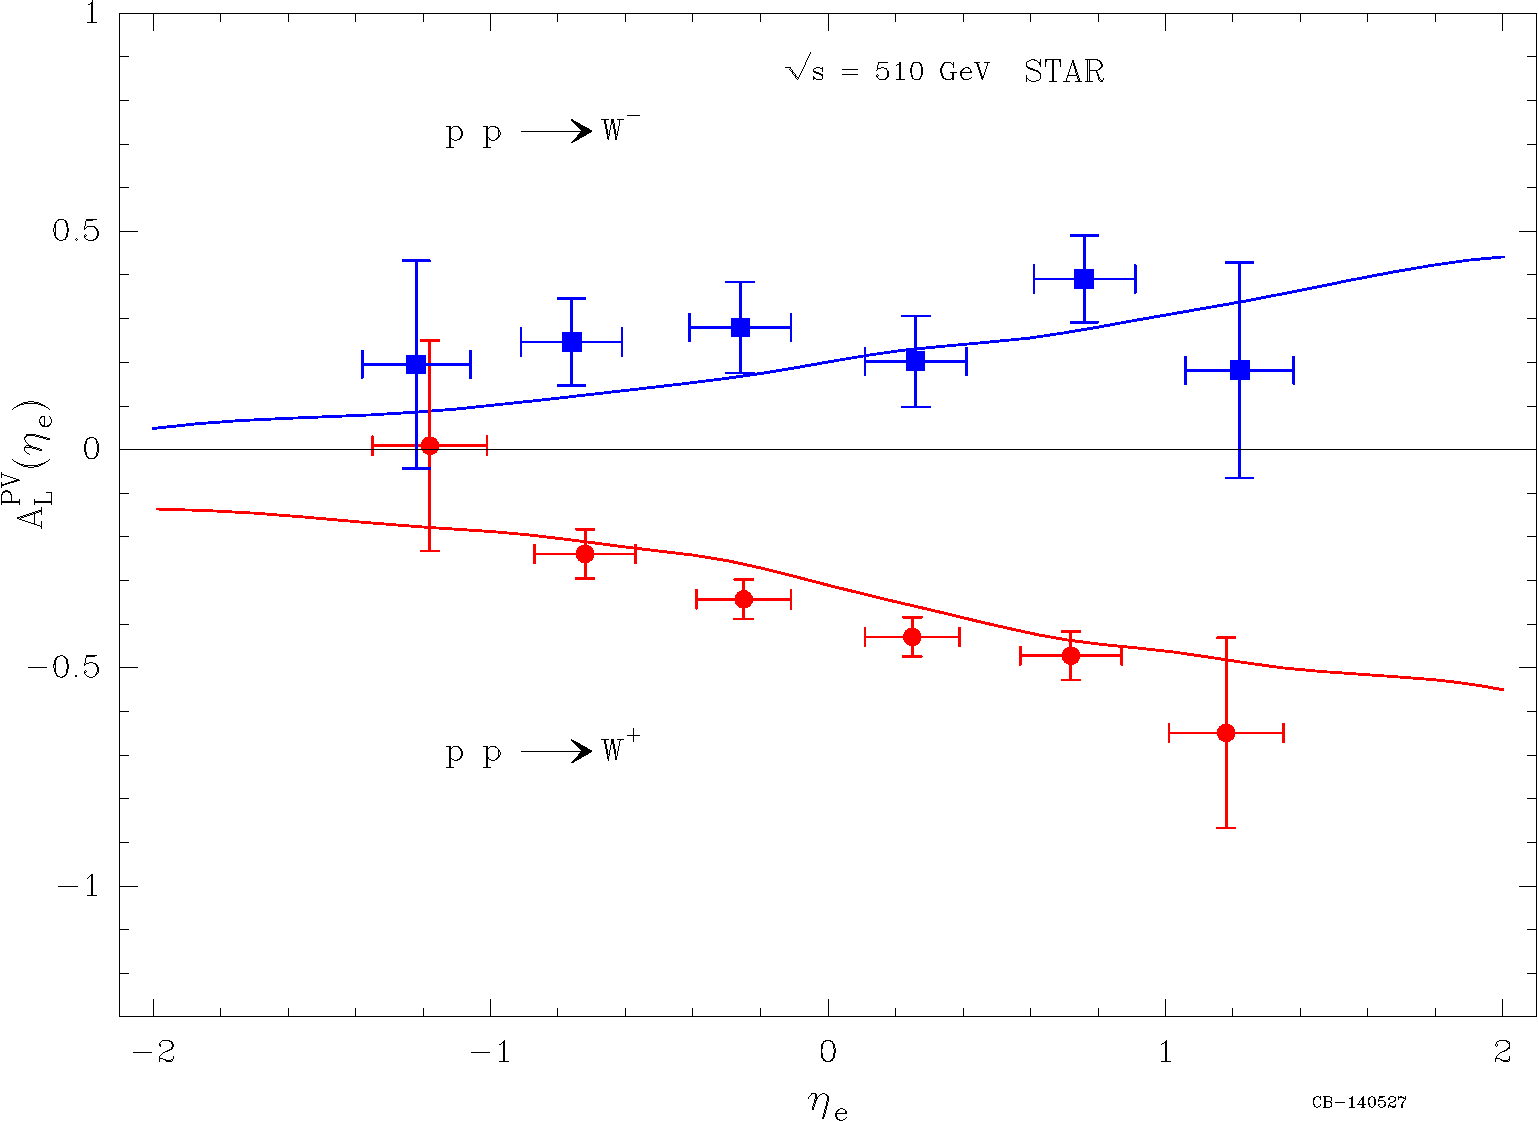
\includegraphics[width=0.70\linewidth]{figs_xj/BBS2008_STARW_submitted.pdf} 
  \caption{\label{fig:STAR_WBBS2008} BBS2008 prediction~\cite{Bourrely2013296}, compared with STAR  $A_L$ data of $W^\pm$ production~\cite{Adamczyk:2014xyw}. }
\end{figure}

%BBS2008 ratios
\begin{figure} [htbp]
  \centering
    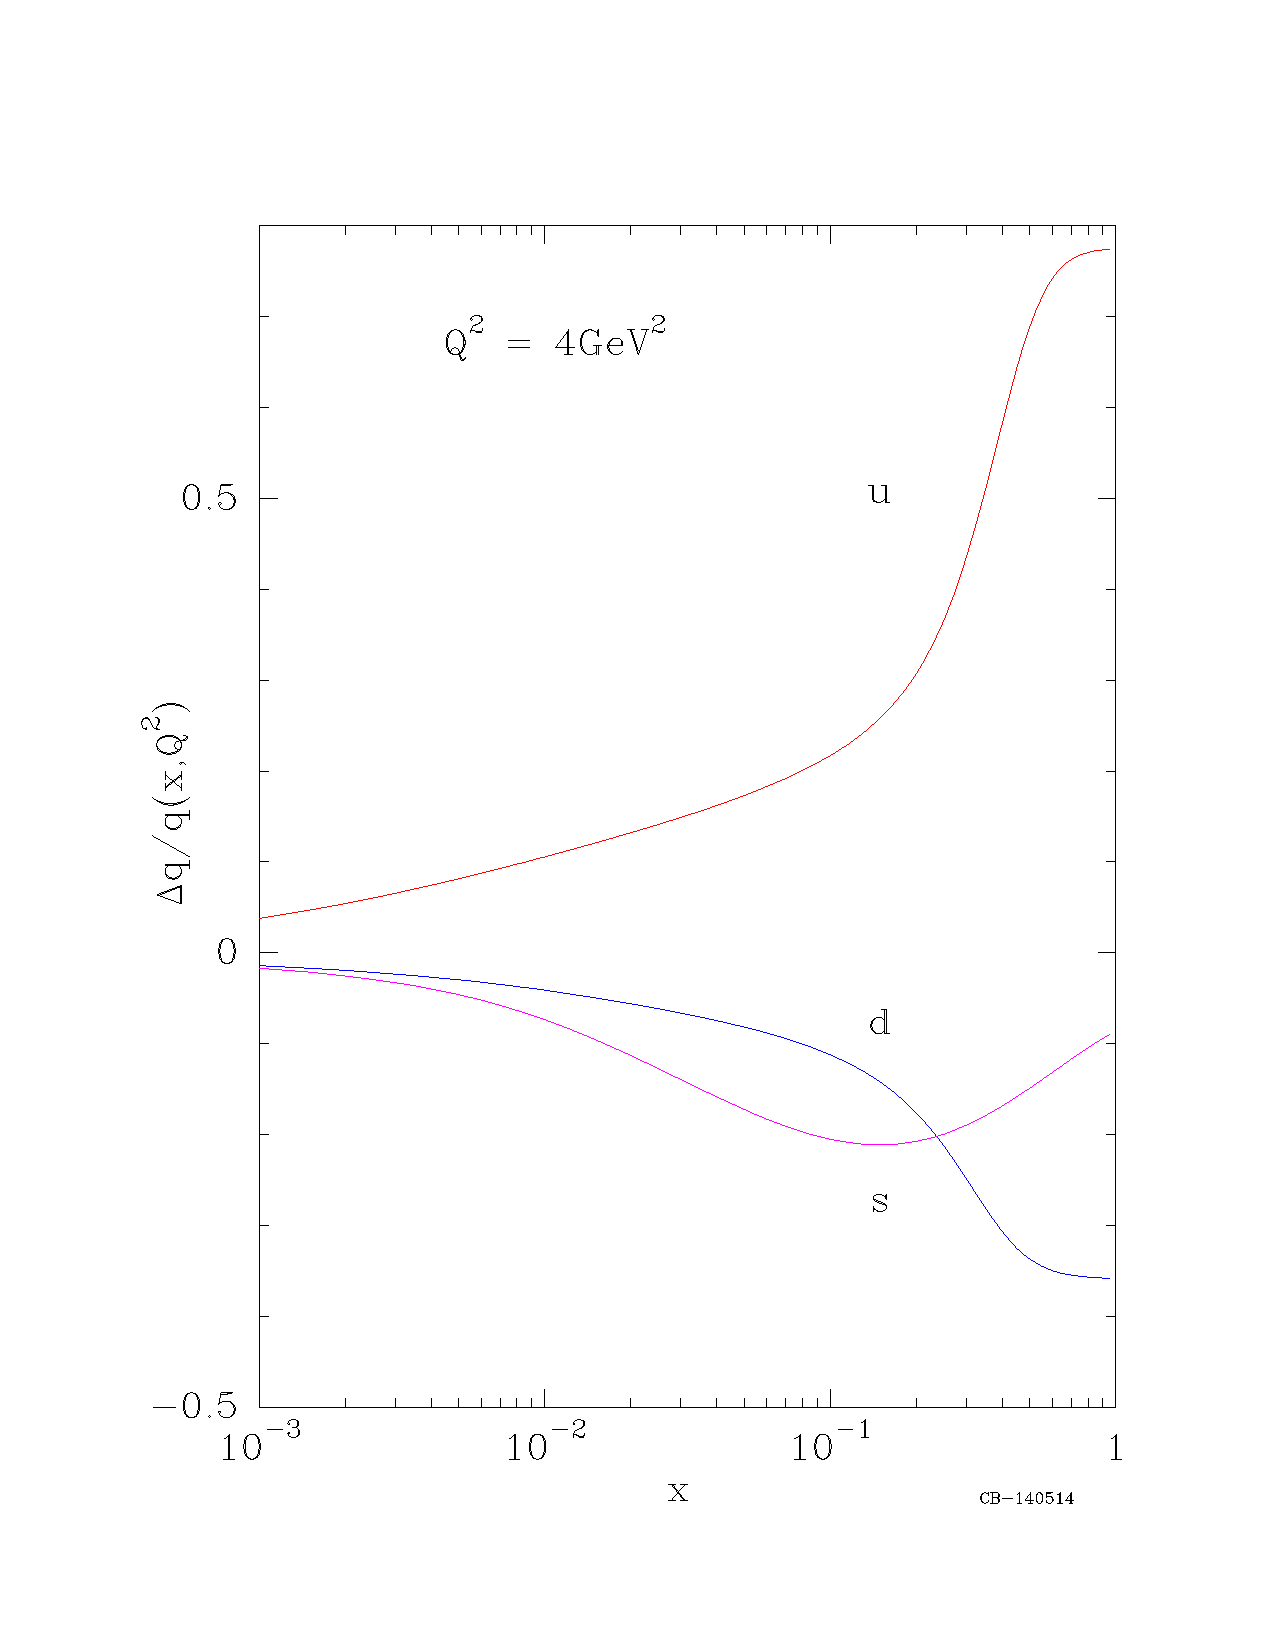
\includegraphics[width=0.49\linewidth]{figs_xj/BBS_deltaqoq.pdf}
    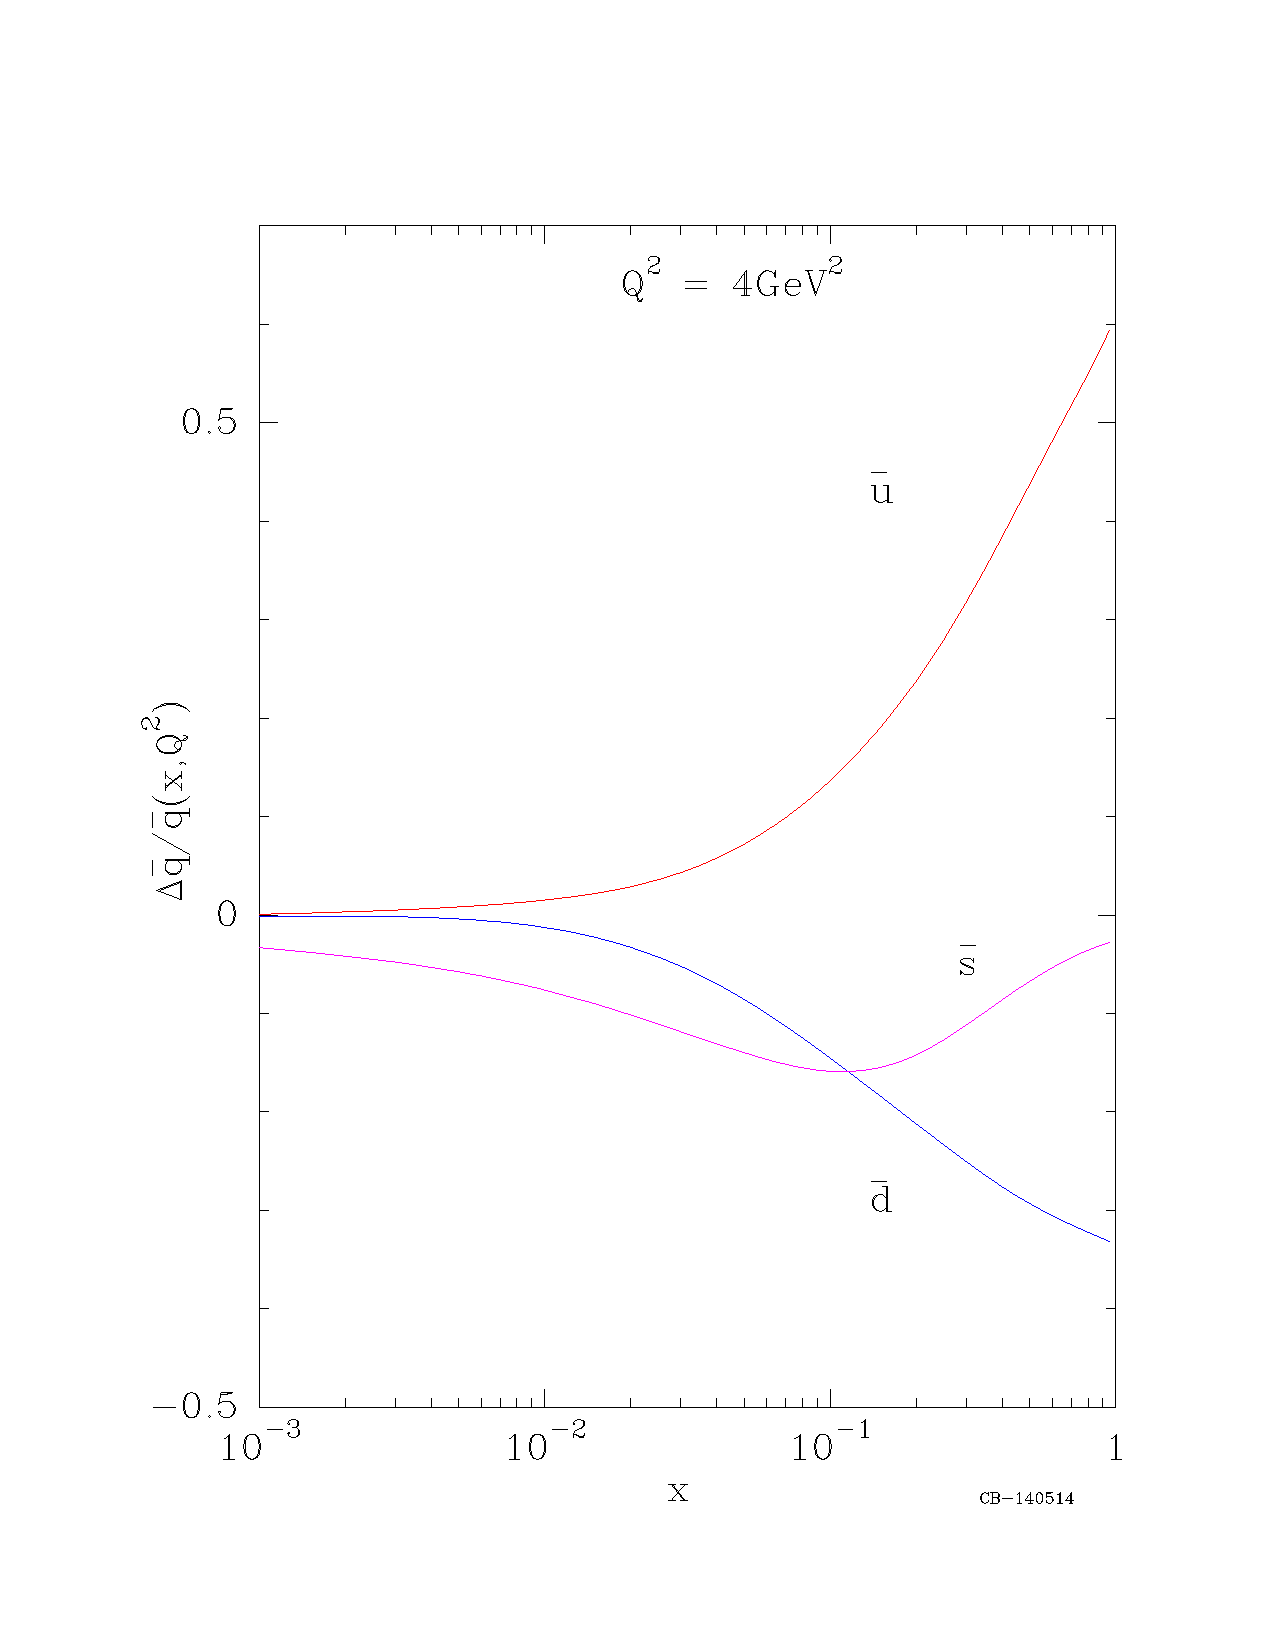
\includegraphics[width=0.49\linewidth]{figs_xj/BBS_deltaqbaroqbar.pdf} \\
  \caption{\label{fig:BBS_deltaqoq} BBS2008 prediction~\cite{Bourrely200739}, of ratio for different quark flavor $\Delta q/q$  (left) and $\Delta \bar{q}/\bar{q}$ at the kinematics of this experiment $Q^2=4.0$ GeV$^2$.  }
\end{figure}

The HERMES data demonstrated that, within the experimental precision, 
the semi-inclusive double-spin asymmetries $A_{1N}^h$ 
at $\langle Q^2 \rangle=2.5$ GeV$^2$ 
agree reasonably well with the 
SMC data~\cite{Adeva:1997qz} at $\langle Q^2 \rangle=10$ GeV$^2$, COMPASS 
asymmetry data on proton and deuteron targets~\cite{Alekseev:2010ub}
averaged at $\langle Q^2 \rangle=10$ GeV$^2$, also agree well with HERMES data.

This non-trivial agreement indicates that semi-inclusive asymmetries have rather weak $Q^2$ dependencies and 
the expected violation of naive \lo $x$-$z$ separation is not large.  
The apparent ``precocious $Q^2$-scaling'' suggests that at a modest $Q^2$, such as at HERMES $\langle Q^2 \rangle=2.5$ GeV$^2$ and 
at $\langle Q^2 \rangle=4.0$ GeV$^2$ for this experiment, information on the  quark distributions and quark polarizations should be reasonably  
well-preserved in semi-inclusive reactions at JLab-12GeV.   Ji, Ma and Yuan have  
explicitly proved~\cite{Ji:2004wu} that QCD factorization is valid for SIDIS with 
hadrons emitted in the current fragmentation region with low  
transverse momentum $p_{\perp h } \ll Q$.  QCD factorization of spin-dependent
cross sections in SIDIS and Drell-Yan has also been proved
 for the low $p_{\perp h }$ case~\cite{Ji:2004xq}.
JLab-6GeV  Hall-C (E00-108) SIDIS  results~\cite{Navasardyan:2006gv, Asaturyan:2011mq}, on unpolarized SIDIS cross section ratios
of proton and deuteron with 5.5 GeV beam and $\langle Q^2 \rangle=2.3$ GeV$^2$,  
also indicated that the leading order naive $x$-$z$ separation is
rather close to the reality. 

% NLO Global fits.

 It was  pointed out by Frankfurt et al.~\cite{LFrankfurt1989141}, Close and Milner~\cite{PhysRevD.44.3691} and by Christova and Leader~\cite{Christova:1999he, Christova:2000nz} that 
if the yield-difference  helicity-asymmetries $A_{1N}^{\pi^+ - \pi^-}$ are measured with  high precision,
quark polarization $\Delta u_v$, $\Delta d_v$ and $\Delta \bar{u} - \Delta \bar{d}$ can be extracted
at \lo independent of the knowledge of fragmentation functions.  Even 
at the \nloo, information on the 
valence quark polarizations is well-preserved in the combined 
asymmetries $A_{1N}^{\pi^+ - \pi^-}$, due to the fact that contributions from 
gluons as well as sea-quarks cancel exactly to all orders of QCD~\cite{Christova:2000nz} in this charge and flavor 
non-singlet combination.
In practice, the combined asymmetry $A_{1N}^{\pi^+ - \pi^-}$ poses more
experimental challenges, since precise knowledge on hadron phase spaces and detection 
efficiencies are required. This experiment,  in JLab-12GeV Hall A with the Super BigBite and BigBite two spectrometer combination,  is specifically designed to measure $A_{1N}^{\pi^+ - \pi^-}$ with well-controlled hadron phase space and detector efficiencies,  
 very different from other SIDIS measurements carried out earlier such as  the HERMES and the  COMPASS experiments,
% and the planned CLAS12, 
this experiment will use two independent magnetic spectrometers. By flipping the magnetic 
polarity of the hadron spectrometer, identical phase spaces between $\pi^+$ and $\pi^-$ 
reaction can be achieved such that the combined asymmetry $A_{1He}^{\pi^+ - \pi^-}$ can be 
determined with high precision.
% in addition to the individual asymmetries $A_{1He}^h$. 
At $Q^2$ of $2.0\sim 6.7$ GeV$^2$, and $x=0.110 \sim 0.600$ ??? xxx.xx , this experiment will 
provide independent precision data on $\Delta d_v -{1 \over 4} \Delta u_v$.
When combined with the expected world data on polarized proton, 
%especially from the planned future CLAS12 experiment, 
to obtain $\Delta u_v - \Delta d_v$,
this experiment will provide the
opportunity to address the polarized sea asymmetry $\Delta \bar{u}- \Delta \bar{d}$. 

At the \nloo, following the well established formalism~\cite{PhysRevLett.101.072001},
tools of NLO QCD global fits, which include data sets from both inclusive and semi-inclusive reactions,
have become available.   As a standard procedure,  such global NLO QCD fit
has also included RHIC $pp$ data~\cite{deFlorian:2014yva}, in forward $\pi^0$ and jet longitudinal double-spin asymmetries $A_{LL}^{\pi^0}$, and $A_{LL}^{jet}$. 
Although there's a reasonable  set of SIDIS  data on proton and deuteron targets, from HERMES and COMPASS experiment, and soon from JLab-6GeV CLAS eg1-dvcs run group,  the world data on SIDIS asymmetries  currently only includes
one $^3$He data set, with rather large error bars, obtained by HERMES in 1996.
The high statistics $^3$He data from this experiment, adding much precise
 neutron SIDIS asymmetries to the world data sample,  
will serve as stringent constraints on pPDFs through NLO global fits~\cite{epjcxj2006}. 
Data from this experiment  will  indirectly constrain  $\Delta g$   through NLO global fit. 
The main source of this sensitivity to $\Delta g$ comes from 
the $Q^2$-evolutions of the inclusive $g_1$ structure function, but now with 
 sea and valence contributions much better
 separated by semi-inclusive data in the global fit~\cite{sassotnlo,epjcxj2006}.
Therefore,  data from this experiment will  independently verify 
the recent claim of a small positive gluon polarization based on RHIC inclusive jet data. 
% cite 2014 STAR jet A_LL here.
%  $A_{LL}^{\pi^0}$ data from PHENIX .

Jefferson Lab Hall A, with its high luminosity polarized $^3$He target, has the unique
advantage in providing high precision neutron asymmetry data in nucleon spin studies. 
In obtaining quark helicity information from neutron,  the Figure-of-Merit of  a polarized $^3He$ target has always been much better than from that of a polarized deuteron target from ND$_3$.
%mention SLAC E154
For example, Hall A data on inclusive  $A_{1n}$ and $d_2^n$ measurements~\cite{A1N_PR}
has improved previous world knowledge by an order of magnitude in each case. 
The Hall A polarized $^3$He target system has been under continuous improvements over 
the last decade.  In 2008-2009, it reached an average in-beam polarization of 60$\%$  
during the Neutron Transversity experiment (E06-010).
A large acceptance magnetic spectrometer, the BigBite spectrometer, with its electron detector package
has been operated successfully in Neutron Transversity and d2n experiments. 
%At 11 GeV beam energy, SIDIS measurement can reach  
%$\langle Q^2 \rangle =4.0$ GeV$^2$ and $\langle W \rangle =3.5$ GeV, at which point the 
%direction of the momentum transfer $\vec q$ is as forward as $6^\circ$. 
%To detect the leading hadron in the current fragmentation regime, the hadron
%spectrometer should be arranged to be directly along $\vec q$. 
The planned Hall A Super-Big-Bite spectrometer with  a large solid angle and a large momentum acceptance, in addition to its unique particle identification Ring Imaging Cherecnkov  detector (RICH), 
in  combination with the high polarization electron beam at 11 GeV, 
a high luminosity and high polarization $^3$He target,  make it possible for a dramatic improvement on the world data set of 
SIDIS neutron asymmetries.


\section{Flavor Asymmetry of Unpolarized and Polarized Sea}
 Fermilab experiment E866 reported measurements of the 
 yield ratio of Drell-Yan muon pairs
 from an 800 GeV/c proton beam incident on hydrogen and deuterium~\cite{e8661,e8662}. 
The data suggested a significantly  asymmetric light sea quark distribution over an 
 appreciable range in $x$; the asymmetry $\bar{d}/\bar{u}$ peaked around $x=0.18$, as shown in Fig.~\ref{fig:e866}.
 Furthermore, based on the E866 data and the CTEQ4M global-fit values of $\bar{u}+\bar{d}$,  
 the values of $\bar{d}(x) - \bar{u}(x)$ were extracted, wit the moment
 $\int_{0}^{1} \left[ \bar{d}(x) - \bar{u}(x) \right]dx = 0.118 \pm 0.012$.
 Many theoretical models, including the meson cloud model, the chiral-quark model,
the Pauli-blocking model, the instanton model, the chiral-quark soliton model and 
the statistical model, have been proposed to explain the $\bar{d}/\bar{u}$ asymmetry.
These models can describe the $\bar{d}-\bar{u}$ reasonably well. However, they all have difficulties 
explaining the $\bar{d}/\bar{u}$ ratio at $x>0.2$.  
%------------------------------------------------------------------
\begin{figure}[htbp]
%\centerline{\psfig{figure=plots/e866_peng2.eps,height=55mm}
%\hspace{0.5cm}\psfig{figure=plots/e866_peng1.eps,height=55mm}}
\centerline{
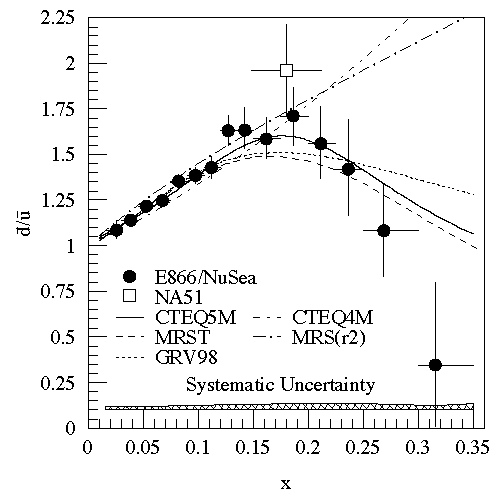
\includegraphics[width=0.50\linewidth]{figs_xj/e866_dbub.pdf}
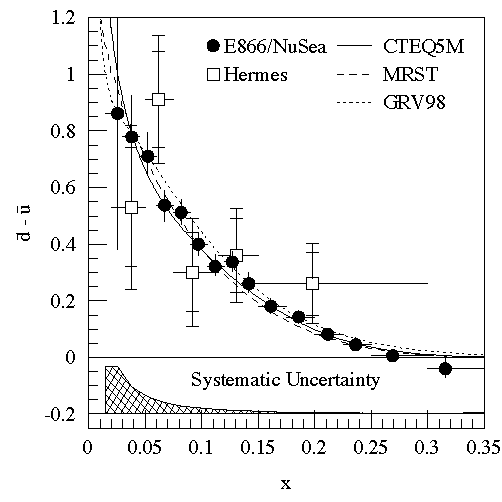
\includegraphics[width=0.50\linewidth]{figs_xj/e866_dmu.pdf}
}
\vspace{-2mm}
\caption{The Fermilab E866 results~\protect\cite{e8661,e8662}. 
The left plot shows the ratio  ${\bar d}/{\bar u}$ as a function of $x$, the right plot 
shows the extracted  value of $\bar{d}(x) - \bar{u}(x)$ together with the HERMES semi-inclusive  
DIS results.
}
\label{fig:e866}
\end{figure}
%-----------------------------------------------------------------

 Since the unpolarized sea demonstrates a significant flavor asymmetry, 
 one naively speculates a sizable flavor asymmetry also exists for 
 the polarized sea in the same $x$-region.
 Indeed, many theory models have specific 
 implications for the spin structure of the nucleon sea. 
For example, the Pauli-blocking model and 
 the instanton model both predict a large asymmetry, 
 $\int_0^1 [\Delta \bar{u}(x)-\Delta \bar{d}(x)]dx={5 \over 3} \cdot \int_0^1 [\bar{d}(x)-\bar{u}(x)]dx \approx 0.2$.
 In the chiral-quark soliton model, $\Delta \bar{u}-\Delta \bar{d}$ appears in leading-order ($N_c^2$) in a large 
$N_c$-expansion, while $\bar{d}-\bar{u}$ appears in the next-to-leading order ($N_c$). 
 On the other hand, those meson cloud models which only include the $\pi$-meson 
predict $\Delta \bar{u}=\Delta \bar{d}=0$ 
 since the sea-quarks reside in a spin-0 $\pi$-meson. By considering a vector meson ($\rho$) cloud, non-zero sea 
 polarization 
 was predicted.
A summary of theoretical
predictions~\cite{jcpengpol} of $I_\Delta = \int_0^1 [\Delta \bar{u}(x)-\Delta \bar{d}(x)]dx$ are given in Table.~\ref{tab:polubdb}. If the
 flavor asymmetry of the polarized sea is indeed as large as the predictions of many models 
shown in Table.~\ref{tab:polubdb}, it would imply that a significant fraction of the Bjorken
sum, $\int_0^1[g_1^p(x)-g_1^n(x)]dx$, comes from the flavor asymmetry of the polarized nucleon sea.
The high statistics $^3$He data from this experiment, together with the expected world proton data, 
will provide us with the first opportunity to discover the asymmetry in the polarized sea.
%-------------------------------------------------------------------------------------------
\begin{table}[htbp]
\begin{center}
%\vspace{-0.5cm}
\begin{tabular}{ccc}
\hline
     Model                    & $I_\Delta$ prediction & Authors and References \\ \hline
    Meson cloud  &  0                    & Eichten {\it et al.}~\protect\cite{eichten},\\ 
    ($\pi$-meson) &                     &  Thomas~\protect\cite{thomas}\\ 
    Meson cloud  &  $\simeq$ $-0.007$ to $-0.027$ & Fries {\it et al.}~\protect\cite{fries} \\ 
    ($\rho$-meson) &   & \\ 
    Meson cloud  & $ =-6 \int_0^1 g_1^p(x)dx \simeq -0.7 $ & Boreskov {\it et al.}~\protect\cite{Boreskov} \\ 
    ($\pi-\rho$ interference) &                         &  \\ 
    Meson cloud & $\simeq$ $-0.004$ to $-0.033$ & Cao {\it et al.}~\protect\cite{cao} \\ 
    ($\rho$ and $\pi-\rho$ interference) &  &  \\ 
    Meson cloud  &  $< 0$                                          & Kumano {\it et al.}~\protect\cite{Kumano} \\ 
    ($\rho$-meson) &                                            & \\ 
    Meson cloud & $\simeq 0.12$ & Fries {\it et al.}~\protect\cite{fries2} \\ 
    ($\pi-\sigma$ interference) & &  \\ 
    Pauli-blocking (bag model)  & $\simeq 0.09$ & Cao {\it et al.}~\protect\cite{cao} \\ 
    Pauli-blocking (ansatz) & $\simeq 0.3$ & Gluck {\it et al.}~\protect\cite{gluck} \\ 
    Pauli-blocking & $={5 \over 3} \int_0^1 [\bar{d}(x)-\bar{u}(x)]dx \simeq 0.2$ & Steffens~\protect\cite{steffens} \\ 
    Chiral-quark soliton & $0.31$ & Dressler~\protect\cite{dressler} \\ 
    Chiral-quark soliton & $\simeq \int_0^1 2 x^0.12[\bar{d}(x)-\bar{u}(x)]dx$ & Wakamatsu {\it et al.}~\protect\cite{wakamatsu} \\ 
    Instanton & $={5 \over 3} \int_0^1 [\bar{d}(x)-\bar{u}(x)]dx \simeq 0.2$ & Dorokhov~\protect\cite{dorokhov} \\ 
    Statistical & $\simeq  \int_0^1 [\bar{d}(x)-\bar{u}(x)]dx \simeq 0.12$ & Bourrely {\it et al.}~\protect\cite{bbs} \\ 
    Statistical & $ >  \int_0^1 [\bar{d}(x)-\bar{u}(x)]dx \simeq 0.12$ & Bhalerao~\protect\cite{bhalerao} \\ 
\hline
 \end{tabular}
\end{center}
\caption{\label{tab:polubdb}
A summary~\protect\cite{jcpengpol} of theoretical
predictions of $I_\Delta = \int_0^1 [\Delta \bar{u}(x)-\Delta \bar{d}(x)]dx$.}
\end{table}
%-------------------------------------------------------------------------------------------



